% !TEX TS-program = XeLaTeX
% use the following command: 
% all document files must be coded in UTF-8
\documentclass{textolivre}
% for anonymous submission
%\documentclass[anonymous]{textolivre}
% to create HTML use 
%\documentclass{textolivre-html}
% See more information on the repository: https://github.com/leolca/textolivre

% Metadata
\begin{filecontents*}[overwrite]{article.xmpdata}
    \Title{Análisis sobre la productividad en torno a la alfabetización informacional en la etapa de Educación Superior}
    \Author{Gerardo Gómez García \sep Francisco Javier Hinojo Lucena \sep Inmaculada Aznar Díaz \sep José María Romero Rodríguez}
    \Language{es}
    \Keywords{Alfabetización informacional \sep TIC \sep Competencia informacional \sep Educación Superior \sep Bibliometría}
    \Journaltitle{Texto Livre}
    \Journalnumber{1983-3652}
    \Volume{14}
    \Issue{2}
    \Firstpage{1}
    \Lastpage{13}
    \Doi{10.35699/1983-3652.2021.33694}

    \setRGBcolorprofile{sRGB_IEC61966-2-1_black_scaled.icc}
            {sRGB_IEC61966-2-1_black_scaled}
            {sRGB IEC61966 v2.1 with black scaling}
            {http://www.color.org}
\end{filecontents*}

% used to create dummy text for the template file
\definecolor{dark-gray}{gray}{0.35} % color used to display dummy texts
\usepackage{lipsum}
\SetLipsumParListSurrounders{\colorlet{oldcolor}{.}\color{dark-gray}}{\color{oldcolor}}

% used here only to provide the XeLaTeX and BibTeX logos
\usepackage{hologo}

% used in this example to provide source code environment
%\crefname{lstlisting}{lista}{listas}
%\Crefname{lstlisting}{Lista}{Listas}
%\usepackage{listings}
%\renewcommand\lstlistingname{Lista}
%\lstset{language=bash,
        breaklines=true,
        basicstyle=\linespread{1}\small\ttfamily,
        numbers=none,xleftmargin=0.5cm,
        frame=none,
        framexleftmargin=0.5em,
        framexrightmargin=0.5em,
        showstringspaces=false,
        upquote=true,
        commentstyle=\color{gray},
        literate=%
           {á}{{\'a}}1 {é}{{\'e}}1 {í}{{\'i}}1 {ó}{{\'o}}1 {ú}{{\'u}}1 
           {à}{{\`a}}1 {è}{{\`e}}1 {ì}{{\`i}}1 {ò}{{\`o}}1 {ù}{{\`u}}1
           {ã}{{\~a}}1 {ẽ}{{\~e}}1 {ĩ}{{\~i}}1 {õ}{{\~o}}1 {ũ}{{\~u}}1
           {â}{{\^a}}1 {ê}{{\^e}}1 {î}{{\^i}}1 {ô}{{\^o}}1 {û}{{\^u}}1
           {ä}{{\"a}}1 {ë}{{\"e}}1 {ï}{{\"i}}1 {ö}{{\"o}}1 {ü}{{\"u}}1
           {Á}{{\'A}}1 {É}{{\'E}}1 {Í}{{\'I}}1 {Ó}{{\'O}}1 {Ú}{{\'U}}1
           {À}{{\`A}}1 {È}{{\`E}}1 {Ì}{{\`I}}1 {Ò}{{\`O}}1 {Ù}{{\`U}}1
           {Ã}{{\~A}}1 {Ẽ}{{\~E}}1 {Ũ}{{\~u}}1 {Õ}{{\~O}}1 {Ũ}{{\~U}}1
           {Â}{{\^A}}1 {Ê}{{\^E}}1 {Î}{{\^I}}1 {Ô}{{\^O}}1 {Û}{{\^U}}1
           {Ä}{{\"A}}1 {Ë}{{\"E}}1 {Ï}{{\"I}}1 {Ö}{{\"O}}1 {Ü}{{\"U}}1
           {ç}{{\c{c}}}1 {Ç}{{\c{C}}}1
}


\journalname{Texto Livre}
\thevolume{14}
\thenumber{2}
\theyear{2021}
\receiveddate{\DTMdisplaydate{2020}{12}{11}{-1}} % YYYY MM DD
\accepteddate{\DTMdisplaydate{2021}{02}{28}{-1}}
\publisheddate{\today}
% Corresponding author
\corrauthor{José María Romero Rodríguez}
% DOI
\articledoi{10.35699/1983-3652.2021.33694}
% list of available sesscions in the journal: articles, dossier, reports, essays, reviews, interviews, editorial
\articlesessionname{dossier}
% Abbreviated author list for the running footer
\runningauthor{Gómez García et al.}
\editorname{Anna Izabella Miranda Pereira}

\title{Análisis sobre la productividad en torno a la alfabetización informacional en la etapa de Educación Superior}
\othertitle{Análise de produtividade em torno do letramento informacional no nível de ensino superior}
\othertitle{Productivity analysis around information literacy in the higher education stage} 
% if there is a third language title, add here:
%\othertitle{Artikelvorlage zur Einreichung beim Texto Livre Journal}

\author[1]{Gerardo Gómez García \orcid{0000-0002-1123-5572} \thanks{Email: \url{gomezgarcia@ugr.es}}}
\author[1]{Francisco Javier Hinojo Lucena~\orcid{0000-0002-9507-4058}~\thanks{Email: \url{fhinojo@ugr.es}}}
\author[1]{Inmaculada Aznar Díaz~\orcid{0000-0002-0018-1150}~\thanks{Email: \url{iaznar@ugr.es}}}
\author[1]{José María Romero Rodríguez~\orcid{0000-0002-9284-8919}~\thanks{Email: \url{romejo@ugr.es}}}

\affil[1]{Universidad de Granada, Facultad de Ciencias de la Educación, Departamento de Didáctica y Organización Escolar, Granada, Andalucía, España.}

\addbibresource{article.bib}
% use biber instead of bibtex
% $ biber tl-article-template

% set language of the article
\setdefaultlanguage{spanish}
\setotherlanguage{portuguese}
\setotherlanguage{english}

% for spanish, use:
%\setdefaultlanguage{spanish}
\gappto\captionsspanish{\renewcommand{\tablename}{Tabla}} % use 'Tabla' instead of 'Cuadro'
\AfterEndPreamble{\crefname{table}{tabla}{tablas}\Crefname{table}{Tabla}{Tablas}}

% for languages that use special fonts, you must provide the typeface that will be used
% \setotherlanguage{arabic}
% \newfontfamily\arabicfont[Script=Arabic]{Amiri}
% \newfontfamily\arabicfontsf[Script=Arabic]{Amiri}
% \newfontfamily\arabicfonttt[Script=Arabic]{Amiri}
%
% in the article, to add arabic text use: \textlang{arabic}{ ... }

% to use emoticons in your manuscript
% https://stackoverflow.com/questions/190145/how-to-insert-emoticons-in-latex/57076064
% using font Symbola, which has full support
% the font may be downloaded at:
% https://dn-works.com/ufas/
% add to preamble:
% \newfontfamily\Symbola{Symbola}
% in the text use:
% {\Symbola }

% reference itens in a descriptive list using their labels instead of numbers
% insert the code below in the preambule:
\makeatletter
\let\orgdescriptionlabel\descriptionlabel
\renewcommand*{\descriptionlabel}[1]{%
  \let\orglabel\label
  \let\label\@gobble
  \phantomsection
  \edef\@currentlabel{#1\unskip}%
  \let\label\orglabel
  \orgdescriptionlabel{#1}%
}
\makeatother
%
% in your document, use as illustraded here:
%\begin{description}
%  \item[first\label{itm1}] this is only an example;
%  % ...  add more items
%\end{description}
 

% custom epigraph - BEGIN 
%%% https://tex.stackexchange.com/questions/193178/specific-epigraph-style
\usepackage{epigraph}
\renewcommand\textflush{flushright}
\makeatletter
\newlength\epitextskip
\pretocmd{\@epitext}{\em}{}{}
\apptocmd{\@epitext}{\em}{}{}
\patchcmd{\epigraph}{\@epitext{#1}\\}{\@epitext{#1}\\[\epitextskip]}{}{}
\makeatother
\setlength\epigraphrule{0pt}
\setlength\epitextskip{0.5ex}
\setlength\epigraphwidth{.7\textwidth}
% custom epigraph - END


% if you use multirows in a table, include the multirow package
\usepackage{multirow}

% add line numbers for submission
%\usepackage{lineno}
%\linenumbers

%\widowpenalties 1 100
%\usepackage{placeins}

\begin{document}
\maketitle

\begin{polyabstract}
\begin{abstract}
En la actualidad, la cantidad de información procedente de la red digital ha proliferado de una forma exponencial, a causa de la llegada de las tecnologías de la información y la comunicación (TIC). Como consecuencia, la necesidad de fomentar una formación en competencias informacionales se presenta como un desafío educativo de cara a afrontar fenómenos desinformativos actuales como es el caso de las \emph{fake news}. En base a esto, en el presente trabajo se analiza desde el contexto internacional la evolución en torno a la productividad sobre alfabetización informacional en la etapa de Educación Superior. Para ello, se hace uso de diferentes indicadores bibliométricos que permiten sistematizar la información procedente de las bases de datos Web of Sciences y Scopus. Los resultados determinaron que la productividad sobre alfabetización informacional se encuentra en una fase de crecimiento, en el que diferentes autores e instituciones procedentes de diferentes lugares del mundo se encuentran publicando sobre este tópico. El estudio arrojó que la principal línea de publicación torna hacia el análisis de percepciones sobre esta competencia en estudiantes universitarios, el estudio sobre la inmersión de este compendio de destrezas en los planes curriculares, así como en la configuración de instrumentos de diferente naturaleza que permita analizar con exactitud este conjunto de habilidades. Por lo tanto, se aboga por la necesidad de continuar profundizando en el la inclusión de este conjunto de habilidades en la globalidad de disciplinas de la enseñanza superior.

\keywords{Alfabetización informacional \sep TIC \sep Competencia informacional \sep Educación Superior \sep Bibliometría}
\end{abstract}

\begin{portuguese}
\begin{abstract}
Atualmente, a quantidade de informação proveniente da rede digital tem proliferado exponencialmente, devido ao advento das tecnologias de informação e comunicação (TIC). Como consequência, a necessidade de promover a formação em competências de informação é apresentada como um desafio educativo para enfrentar os atuais fenômenos desinformativos, tais como notícias falsas. Com base nisso, este artigo analisa a partir do contexto internacional a evolução da produtividade do letramento da informação na fase do Ensino Superior. Para esse fim, são utilizados diferentes indicadores bibliométricos para sistematizar a informação da Web of Sciences e das bases de dados Scopus. Os resultados determinaram que a produtividade no letramento da informação está numa fase de crescimento, em que diferentes autores e instituições de diferentes partes do mundo estão publicando sobre esse tema. O estudo mostrou que a principal linha de publicação se volta para a análise das percepções sobre essa competência nos estudantes universitários, o estudo sobre a imersão desse compêndio de competências nos planos curriculares e a configuração de instrumentos de natureza diferente que permitem a análise exata desse conjunto de competências. Por conseguinte, advoga-se a necessidade de continuar a aprofundar a inclusão desse conjunto de competências na globalidade das disciplinas do ensino superior.

\keywords{Letramento da Informação \sep TIC \sep Competências de informação \sep Ensino superior \sep Bibliometria}
\end{abstract}
\end{portuguese}

\begin{english}
\begin{abstract}
Today, the amount of information coming from the digital network has proliferated exponentially, due to the advent of information and communication technologies (ICT). As a result, the need to promote training in information competences is an educational challenge in the face of current disinformation phenomena such as fake news. Therefore, this paper analyses the evolution of information literacy productivity in higher education from an international context. For this purpose, different bibliometric indicators were used to systematize the information from the Web of Sciences and Scopus databases. The results showed that information literacy productivity is in a growth phase, with different authors and institutions from different parts of the world publishing on this topic. The study showed that the main line of publication turns towards the analysis of perceptions of this competence in university students and the study of the immersion of this compendium of skills in the curricular plans, as well as the configuration of instruments of a different nature that allows analyzing exactly this set of skills. Such results, therefore, suggest the need for keeping the inclusion of this skill set in the globality of higher education disciplines.

\keywords{Information literacy \sep ICT \sep Information competence \sep Higher education \sep Bibliometrics}
\end{abstract}
\end{english}

% if there is another abstract, insert it here using the same scheme
\end{polyabstract}


\section{Introducción}\label{intro}
En los últimos años, la sociedad se encuentra en una fase de cambio, asociado a la irrupción de las Tecnologías de la Información y la Comunicación (TIC), que han provocado un cambio abrupto en la forma de llevar a cabo nuestros procesos cotidianos. Con la llegada de este medio a nuestras vidas, la actual Sociedad de la Información se caracteriza por una accesibilidad inmediata hacia la información, así como por priorizar como lugares de búsqueda de información webs digitales y redes sociales como principales fuentes de información a consultar para informarse \cite{alfonso2019}. %(ALFONSO, GALERA Y CALVO, 2019).

Como consecuencia, esto ha ocasionado que se vuelva más compleja la vinculación existente entre el individuo y la información, ya que la aparición de las redes ha abierto la posibilidad a difundir masivas cantidades de información de forma instantánea a una infinidad de usuarios digitales \cite{alonsoelat2020}. %(ALONSO ET AL, 2020). 
Lo cual provoca que numerosas noticias falsas, conocidas como \emph{fakes news}, hayan irrumpido en la población, causando un sentimiento de confusión y disrupción en la sociedad \cite{lopez-borrull2018}. %(LÓPEZ BORRUL et al, 2018).

En el marco de esta sociedad, y frente a esta situación que preocupa a la ciudadanía, resulta preciso formar a las futuras generaciones para que posean competencias de buscar, evaluar y seleccionar diversas fuentes de información, con la finalidad de discernir cuáles son pertinentes de calidad y cuáles no lo son. La adquisición de competencias en información, entendidas como el resultado del proceso de alfabetización informacional resulta imprescindible para el desarrollo individual y colectivo de la sociedad en su conjunto \cite{alonso-varela2020}. %(ALONSO Y SARAIVA, 2020).

En relación con este proceso, la alfabetización informacional queda entendida como el conjunto de habilidades y competencias que todos los individuos necesitan para realizar un determinado desempeño con la información. Entre las capacidades que se hallan inmersas en este concepto, se encuentra el pensamiento crítico, así como la comprensión ética del uso de la información con respecto a sus implicancias políticas \cite{torrell2020}. %(TORRELL, 2020).

De acuerdo con la \cite{oecd2017}, %OCDE (2017), 
la implementación de la alfabetización informacional en los centros educativos garantizará el derecho a cada estudiante a aprender diversas normas para expresar la información, gestionar fuentes de forma adecuada o evaluar su veracidad. Esto implicará, por lo tanto, un mejor uso de la red y de las TIC.

Así, la trascendencia de la alfabetización informacional radica en cumplimentar diferentes objetivos: promover la mejora continua del proceso de aprendizaje; discriminar la calidad de la información para identificar aquellas características que convierten una fuente en veraz o no; formar personas críticas y competentes en una sociedad plagada de información, y evitar, por lo tanto, el fenómeno de compartir de forma masiva noticias falsas que provoquen un sentimiento de confusión en la ciudadanía \cite{balcer2020, klucevsek2017}. %(BALCER, 2020; KLUCEVSEK, 2017).

En este sentido, la \cite{unesco2016} %UNESCO (2016) 
considera imprescindible la formación de la ciudadanía en alfabetización mediática e informacional, en orden de garantizar su desarrollo en la sociedad. Tal es así que sitúa la evaluación de la información como una herramienta fundamental para el pleno desenvolvimiento de los individuos en las sociedades democráticas.

En torno a estos conceptos y, en general, a la trascendencia de la competencia informacional en las aulas de Educación Superior, son múltiples los trabajos que discuten sobre la importancia de este compendio de destrezas en esta etapa educativa, así como en la necesidad de su inclusión en los planes curriculares, como una materia de carácter transversal, común y generalizable a todos las formaciones académicas \cite{waltz2020}. %(WALTZ, MOBERLY Y CARRIGAN, 2020). 
Por un lado, se disciernes investigaciones que se han encargado de comprobar la eficacia de acciones formativas basadas en la adquisición de herramientas para la alfabetización informacional en estudiantes de diferentes disciplinas del conocimiento \cite{ball2019, george2019, lantz2019, sanches2019}. %(BALL, 2019; GEORGE Y ROWLAND, 2019; LANTZ Y DEMPSEY, 2019; SANCHES, 2019). 
Entre las poblaciones que más se analizaron a la hora de evaluar este compendio de destrezas, se encuentran los profesionales de la enseñanza, que han presentado, en términos generales, un nivel promedio \cite{oliveira2019, godbey2018, bougatzeli2015}. %(OLIVEIRA, LOPES Y SPEAR-SWERLING, 2019; GODBEY, 2018; BOUGATZELI, TOGIA Y PAPADIMITRIOU, 2015). 
Los resultados obtenidos indicaron, en la mayoría de los casos, una mejoría en las habilidades de búsqueda, evaluación y selección de la información por parte de los estudiantes. Constructos como la autoeficacia presentada por cada sujeto a la hora de desempeñar habilidades informacionales protagonizan las líneas de múltiples trabajos en la literatura científica \cite{demeulemeesteretal2019, demeulemeester2018}. %(DE MEULEMEESTER ET AL, 2018; DE MEULEMEESTER, BUYSSE Y PELEMAN, 2018).

Por otro lado, se encuentran varios estudios que se encargaron de analizar los factores incidentes en el desarrollo de la alfabetización informacional, como fue el caso del género \cite{pinto2019}, %(PINTO, SALES Y FERNÁNDEZ, 2019), 
la inteligencia emocional \cite{soroya2020}, %(SOROYA ET AL, 2020), 
lugar de trabajo \cite{ahmad2020} %(AHMAD, WIDÉN Y HUVILA, 2020) 
o el uso y familiarización con las TIC \cite{lorenz2019}. %(LORENZ, ENDBERG Y BOS, 2019).

En base a estas evidencias, se observa la creciente presencia de las competencias informacionales dentro del panorama formativo actual. Es por ello que resulta preciso identificar los principales focos de productividad sobre esta línea temática y localizar cual es el estado actual de este tópico dentro de la comunidad científica. A partir de esta idea, el objetivo principal es analizar el nivel de productividad actual en la literatura científica sobre alfabetización informacional en la etapa de Educación Superior. En torno a este propósito, se derivan las siguientes preguntas de investigación:

\begin{itemize}
    \item PI.1: ¿Cuál es el nivel de productividad actual sobre alfabetización informacional en los principales repositorios de datos?
    \item PI.2: ¿Cuáles son las principales revistas que publican sobre este tópico?
    \item PI.3: ¿Cuáles son las instituciones más relevantes en nivel de productividad sobre esta línea de investigación?
    \item PI.4: ¿Cuáles son los autores más prolíficos en este tópico?
    \item PI.5: ¿Cuáles son las principales temáticas que abordan los autores sobre esta temática?
    \item PI.6: ¿Cuáles son los descriptores clave más utilizados por los autores para enmarcar su trabajo?
\end{itemize}

\section{Metodología}
El estudio presenta una visión general y exhaustiva de la investigación acerca de la productividad sobre alfabetización informacional hasta la fecha en la etapa de Educación Superior. Para ello, el trabajo se enmarca dentro de la metodología bibliométrica \cite{vaneck2014, cruz1999, fernandezcano1999}, %(VAN ECK ET AL, 2014; CRUZ, 1999; FERNÁNDEZ-CANO, & BUENO, 1999), 
que, entre otros, se encarga de identificar los siguientes objetivos:

%\begin{itemize}
\begin{enumerate}[label={\alph*}]
    \item Identificar la tendencia de desarrollo de la publicación a través del tiempo en el campo de investigación;
    \item Reconocer las revistas, autores e instituciones más prolíficos en esta temática;
    \item Identificar cuáles son las temáticas más frecuentadas en los artículos.
    \item Determinar cuáles son las palabras clave más utilizadas por los autores que producen sobre alfabetización informacional.
\end{enumerate}
%\end{itemize}

De esta forma, este diseño metodológico da respuesta a las preguntas de investigación planteadas con anterioridad, así como pretende contribuir al campo de la investigación desde varios aspectos. En primer lugar, proporciona a los expertos sobre educación una visión acerca del actual estado de la línea de investigación sobre alfabetización informacional en la enseñanza universitaria. En segundo lugar, permite localizar los focos de productividad sobre esta línea de investigación, de cara a fomentar la colaboración y las redes nodales de desarrollo entre instituciones. Por último, presenta una visión general de cuál ha sido la evolución de la línea temática, pudiéndose detectar aquellos cambios y modificación a lo largo de los años.

\subsection{Recopilación de datos}
La búsqueda y localización de los trabajos científicos tuvieron lugar en el mes de agosto del año 2020. Para garantizar la selección de trabajos científicos de alta calidad, se consideraron únicamente los trabajos en formato artículo, debido a la revisión por pares que llevan a cabo las revistas científicas. Las bases de datos seleccionadas fueron Web of Sciences y Scopus, puesto que gozan de reconocimiento internacional y estándares de calidad. Además de estas bases de datos, se incluyeron distintos índices como fue en el caso de Web of Sciences, en el que se analizaron los índices Sci-Expanded, Ssci, A\&Hci, Cpci-S, Cpci-Ssh, Bkci-S, Bkci-Ssh, Esci, Ccr-Expanded, Ic.

A continuación, se propusieron los criterios de inclusión y exclusión especificados en la \Cref{tab1}, con el propósito de ahondar más en los objetivos de la investigación. Para establecer el dictamen de estos, se tomaron como referentes estudios bibliométricos previos de relevancia dentro del panorama educativo \cite{moreno-guerrero2020, hinojo-lucena2019}. %(MORENO, GÓMEZ-GARCÍA, LÓPEZ, RODRÍGUEZ, 2020; HINOJO, AZNAR, TRUJILLO, CÁCERES Y ROMERO, 2019).

\begin{table}[htpb]
\caption{Criterios de inclusión y exclusión}
\label{tab1}
\scriptsize
\begin{tabular}{p{0.47\textwidth}p{0.47\textwidth}}
\toprule 
Criterios de inclusión (C.I.) & Criterios de exclusión (EX)
\\
\midrule
C.I.1: Artículo de revista & EX1: Capítulos de libro, libros u otros formatos de publicación.
\\
C.I.2: Artículos científicos desde su origen hasta el año 2019 & EX2: No se contemplan los artículos del año 2020 al no ser un año aún acabado
\\
\bottomrule
\end{tabular}
\source{Elaboración propia.}
\end{table}

Para la realización de la investigación, en primer lugar, los descriptores fueron comprobados a través del Thesauro Eric y Unesco para garantizar que su utilización era la idónea para acaparar la mayor cantidad de documentos posibles. La búsqueda fue realizada utilizando los descriptores clave “Information Literacy” AND “Higher Education”  OR “Further Education”.

De esta forma, el siguiente diagrama de flujo explica cómo fue llevado a cabo el procedimiento de escrutinio de los trabajos científicos localizados tras la aplicación de los criterios pertinentes (\Cref{fig1}).

\begin{figure}[h!]
 \centering
 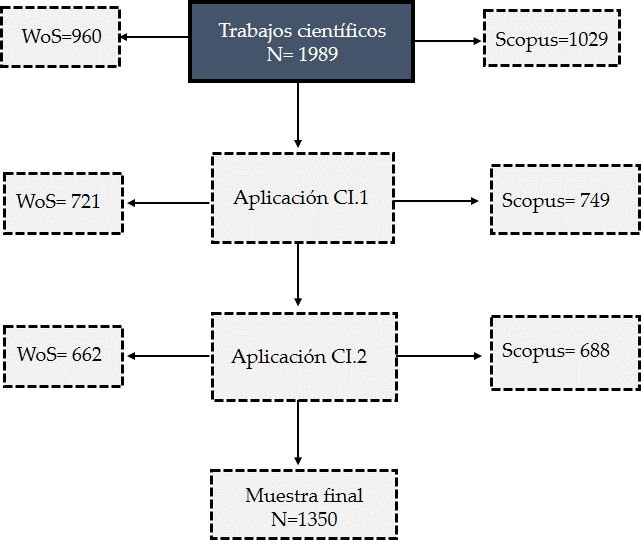
\includegraphics[width=0.5\textwidth]{fig1.png}
 \caption{Diagrama de flujo sobre el proceso de escrutinio de documentos.}
 \label{fig1}
 \source{Elaboración propia.}
\end{figure}

Como resultado se obtuvo una muestra de artículos de X (n=1350), con los que se procedió al análisis. Este fue llevado a cabo a través del paquete bibliometrix del software R.Studio \cite{aria2017}, %(ARIA Y CUCCURULLO, 2017), 
que permite analizar exhaustivamente los documentos en torno a algoritmos estadísticos  que proporcionan información en torno a diferentes indicadores bibliométricos.

\section{Resultados}
\subsection{Productividad diacrónica de la línea de investigación}
En primer lugar, se observa la productividad diacrónica de los documentos publicados desde el origen de la temática, en el año 1995, hasta el año 2019. Tal y como muestra la \Cref{fig2}, el crecimiento en la productividad sobre alfabetización informacional en la etapa de Educación Superior ha sido considerable desde su origen. Se distinguen diferentes tendencias de crecimiento y decrecimiento a lo largo de los años, destacando su ascenso especialmente en los últimos cinco años, en los que los índices de producción han superado los 40 trabajos científicos publicados al año.  En este sentido, y tomando como referencia la ley de Price sobre crecimiento exponencial de la información científica \cite{price1986}, %(PRICE, 1986), 
se observa que el crecimiento desde el origen a los 10 años próximos se ha duplicado, y así sucesivamente, por lo que se podría afirmar que la tendencia de producción se encuentra todavía en apogeo, hasta que, finalmente, acabe en una fase de crecimiento lineal. Asimismo, se observa, que, en general, la cantidad observada en las dos bases de datos son similares, siendo ligeramente superior la encontrada en Scopus.

\begin{figure}[htbp]
 \centering
 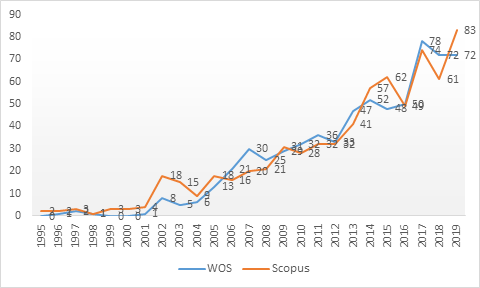
\includegraphics[width=0.6\textwidth]{fig2.png}
 \caption{Productividad diacrónica sobre alfabetización informacional en Educación Superior}
 \label{fig2}
 \source{Elaboración propia.}
\end{figure}

\subsection{Revistas, autores e instituciones más prolíficas
}
En cuanto a las revistas más prolíficas dentro de este campo de investigación, la \Cref{tab2} presenta las 10 primeras revistas que más publican sobre alfabetización informacional en Educación Superior en WoS y Scopus. Cabe destacar que todas ellas reúnen más de 10 documentos, lo cual hace que se consideren como revistas especializadas  sobre la temática de alfabetización informacional, y por lo tanto, constituya uno de los principales fuentes de artículos científicos sobre esta línea temática. Destacan especialmente, en ambos repositorios, revistas como \emph{Reference Services Review}, acumulando más de 50 artículos, y con un índice de impacto muy alto. Le siguen revistas como \emph{Communications in Information Literacy}, \emph{Journal of Information Literacy} o \emph{Journal of Academic Librarianship}, las cuales se caracterizan por poseer un considerable número de citas, y por ende, de impacto.

\begin{table}[h]
\caption{Revistas más prolíficas}
\label{tab2}
\centering
\scriptsize
\begin{tabular}{%
    >{\raggedright\arraybackslash}p{0.3\textwidth}%
    p{0.06\textwidth}%
    p{0.04\textwidth}%
    >{\raggedright\arraybackslash}p{0.3\textwidth}%
    p{0.06\textwidth}%
    p{0.04\textwidth}}
\toprule 
& \multicolumn{2}{c}{WOS} & & \multicolumn{2}{c}{Scopus}
\\
Revista	& Nº Doc & Citas & Revista & Nº Doc & Citas
\\
\midrule
\arrayrulecolor[gray]{.7}
Reference Services Review & 50 & 404 & Reference Services Review & 57 & 766
\\
%\midrule
Journal of Academic LibrarianShip & 47 & 537 & Communications in Information Literacy & 44 & 422
\\
%\midrule
Communications in Information Literacy & 39 & 281 & Journal of Information Literacy & 40 & 143
\\
%\midrule
Portal Libraries and the Academy & 35 & 461 & Journal of Academic Librarianship & 36 & 577
\\
%\midrule
College and Research Libraries & 23 & 385 & Portal & 26 & 313
\\
%\midrule
Chandos Information Professional Series & 22 & 385 & College and Research Libraries & 17 & 307
\\
%\midrule
Collegue Undergraduate Libraries & 15 & 117 & College and Undergraduate Libraries & 17 & 146
\\
%\midrule
Journal of Librarianship and Information Science & 14 & 207 & Communications in Computer and Information Science & 13 & 27
\\
%\midrule
Evidence Based Library and Information Practice & 12 & 18 & Library Review & 12 & 103
\\
%\midrule
Journal of Library Administration & 10 & 56 & Journal of Library Administration & 11 & 85
\\
\arrayrulecolor{black}
\bottomrule
\end{tabular}
\centering
\source{Elaboración propia.}
\end{table}

En cuanto a las instituciones que mayor índice de productividad presentan, la \Cref{tab3} refleja las 10 más prolíficas en la actualidad. Destacan por encima del resto, la \emph{University Libraries}, la \emph{Universidad de Granada} y \emph{California State University}. Sin embargo, atendiendo al índice de impacto de las publicaciones, se hallaron instituciones como \emph{Pennsylvania Commonwealth System of Higher Education}, \emph{Queensland University of Tecnhology Qut} o \emph{University of Scheffield}  cuyos índices de citación por documento son muy elevados.

\begin{table}[h]
\caption{Instituciones más prolíficas}
\label{tab3}
\centering
\scriptsize
\begin{tabular}{%
    >{\raggedright\arraybackslash}p{0.2\textwidth}%
    p{0.06\textwidth}%
    p{0.06\textwidth}%
    p{0.06\textwidth}%
    >{\raggedright\arraybackslash}p{0.2\textwidth}%
    p{0.06\textwidth}%
    p{0.06\textwidth}%
    p{0.06\textwidth}}
\toprule 
& \multicolumn{3}{c}{WOS} & & \multicolumn{3}{c}{Scopus}
\\
Institución	& NºDoc & Citas & Impacto & Institución & NºDoc & Citas & Impacto
\\
\midrule
\arrayrulecolor[gray]{.7}
Universidad de Granada & 25 & 244 & 9.76 & University of Scheffield & 9 & 227 & 25.2
\\
%\midrule
Purdue University & 18 & 81 & 4.5 & Universidad de Granada & 9 & 34 & 3.87
\\
%\midrule
Pennsylvania Commonwealth System of Higher Education & 17 & 240 & 14.11 & Pontificia Universidad Javeriana & 6 & 10 & 1.67
\\
%\midrule
State University System of Florida & 17 & 121 & 7.11 & State University of New York Suny System & 6 & 76 & 12.67
\\
%\midrule
California State University System & 14 & 166 & 11.86 & State University System of Florida & 6 & 42 & 7
\\
%\midrule
University of Sheffield & 10 & 229 & 22.9 & Universidad Distrital Francisco José De Caldas & 5 & 7 & 1.4
\\
%\midrule
Queensland University of Tecnhology Qut & 9 & 146 & 16.22 & The Ohio State University & 5 & 35 & 7
\\
%\midrule
Nevada System of Higher Education & 8 & 64 & 8 & University at Albany & 5 & 67 & 13.4
\\
%\midrule
University of Illinois System & 8 & 20 & 2.5 & California State University System & 4 & 26 & 6.5
\\
\arrayrulecolor{black}
\bottomrule
\end{tabular}
\centering
\source{Elaboración propia.}
\end{table}

Atendiendo a los autores más productivos (\Cref{tab4}), destaca especialmente “Pinto, M.”, que cuenta con un total de 13 aportaciones sobre el tópico, publicados en un amplio periodo de tiempo. Tras este le siguen autores con cinco y cuatro aportaciones respectivamente, procedentes de diferentes instituciones, la mayoría situadas en Estados Unidos, seguido de España.

\begin{table}[h]
\caption{Autores más prolíficos}
\label{tab4}
\centering
\scriptsize
\begin{tabular}{%
    p{0.12\textwidth}%
    p{0.15\textwidth}%
    p{0.08\textwidth}%
    p{0.08\textwidth}%
    >{\raggedright\arraybackslash}p{0.4\textwidth}}
\toprule 
Autor & Nº Documentos & Citas & Impacto & Universidad
\\
\midrule
\arrayrulecolor[gray]{.7}
Pinto, M & 23 & 155 & 6.73 & Universidad de Granada (España)
\\
Maybee, C &	11 & 25 & 2.27 & Purdue University (USA)
\\
Sales, D & 6 & 36 & 6 & Universitat Jaume I (Spain)
\\
Oakleaf, M & 6 & 266 & 44.3 & Syracuse University (USA)
\\
Scott, R & 5 & 30 & 6 & University of Menphis (USA)
\\
Corralls, S & 5 & 129 & 4 & University of Pittsburgh (USA)
\\
Badke, W & 5 & 67 & 13.4 & Trinity Western University (USA)
\\
Jacobson, T & 4 & 64 & 16 & University at Albany
\\
Julien, H & 4 & 8 & 2 & University at Buffalo (USA)
\\
Lupton, M & 4 & 82 & 20.5 & Queensland University of Technology (Australia)
\\
\arrayrulecolor{black}
\bottomrule
\end{tabular}
\centering
\source{Elaboración propia.}
\end{table}



%\FloatBarrier
\subsection{Análisis de términos más frecuentados en abstracts}
Atendiendo a las principales temáticas de los artículos, se procedió a revisar los abstract de todos los manuscritos que compusieron la muestra de la investigación. Se realizó este procedimiento a través de la utilización del software \emph{VosViewer} que permitió analizar las palabras más frecuentadas en los abstract de los trabajos (\Cref{fig3}). Por un lado, una parte de los estudios se trata de investigaciones de carácter empírico que analizaron percepciones sobre alfabetización informacional a diferentes tipos de poblaciones, entre las que frecuentan estudiantes de distintas titulaciones de Educación Superior. Especialmente, el concepto de alfabetización informacional queda englobado dentro de la evaluación y búsqueda de informaciones dentro de la red digital. Asimismo, estos estudios también analizan este constructo a través de la perspectiva de diferentes perspectivas socio-demográficas, como pueden ser el género, la edad, la titulación o la formación previa.

En consiguiente, se encuentran investigaciones que se encargaron de configurar un marco teórico sobre la alfabetización informacional en diferentes disciplinas del conocimiento, como el caso de la ingeniería, la educación o en biblioteconomía. Este tipo de estudios de carácter teórico pretenden evaluar la posible inmersión de la alfabetización informacional dentro de los variados planes curriculares existentes en diferentes ramas del conocimiento, especialmente, desde el contexto bibliotecario.

Otra parte relevante de la literatura científica hace alusión a propuestas de instrumentos que se encargan de medir competencias informacionales asociadas a la alfabetización informacional. Entre los más relevantes destacan la configuración de cuestionarios, asociados no solamente a este constructo, sino también a otros como es el caso de la motivación, el pensamiento crítico o la autoeficacia. Del mismo modo, también se encuentran diferentes trabajos que elaboran rúbricas de evaluación de competencias informacionales. Así lo corrobora en el mapa de descriptores clave la aparición de términos como “survey”, “test”, “rubrique”.

\begin{figure}[h!]
 \centering
 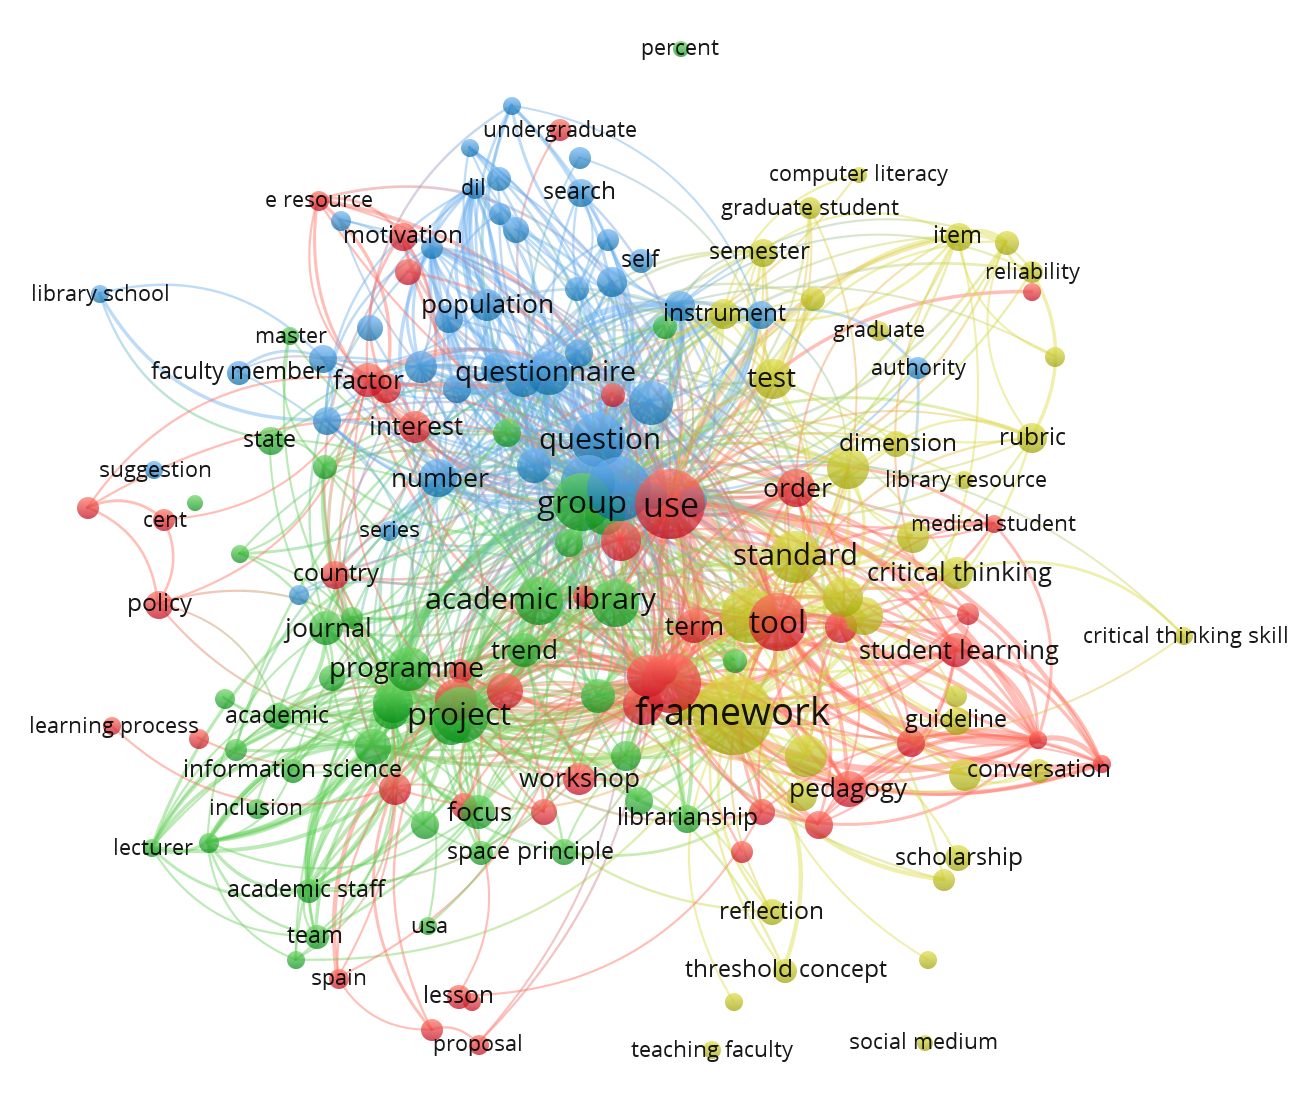
\includegraphics[width=0.8\textwidth]{fig3.png}
 \caption{Descriptores más repetidos en los abstract de los artículos}
 \label{fig3}
 \source{Elaboración propia.}
\end{figure}

\subsection{Evolución de la temática}
Para analizar la evolución que presenta la línea de investigación se recurrió al análisis por co-ocurrencias mediante el algoritmo de \emph{clustering}, localizando los temas de investigación, mostrándose así las palabras clave fuertemente relacionadas. Diferentes constructos se dilucidaron vinculados a la alfabetización informacional (information literacy) como \emph{academic libraries} o \emph{web 2.0.} que tuvo su duración durante los años 1995-2014 a términos presentes como \emph{online learning}, \emph{teaching} o \emph{academic libraries} (\Cref{fig4}).

\begin{figure}[h!]
 \centering
 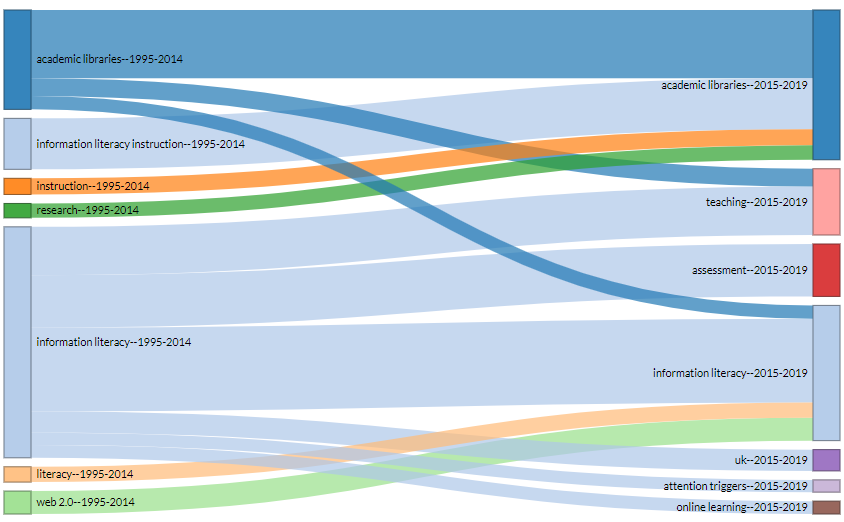
\includegraphics[width=\textwidth]{fig4.png}
 \caption{Evolución cronológica de la temática}
 \label{fig4}
 \source{Elaboración propia.}
\end{figure}

\subsection{Palabras clave más frecuentadas por los autores}
Por último, se profundizó en conocer las palabras clave más repetidas por los autores que han publicados artículos sobre alfabetización informacional (\Cref{fig5}). El análisis de los documentos permitió conocer que los descriptores más encontrados quedaron asociados a la rama educativa como son “education”, “Teaching”, “Students”, “Higher Education”. Además, se encuentran palabras clave vinculadas a diferentes campos del conocimiento como “information science”, “medical education”, “library sciences”, “nursing”, “engineering education” o  “computer sciences”. Por último, se localizan conceptos vinculados a métodos de investigación como “human experiment”, “surveys” o “questionnaries”.

\begin{figure}[h!]
 \centering
 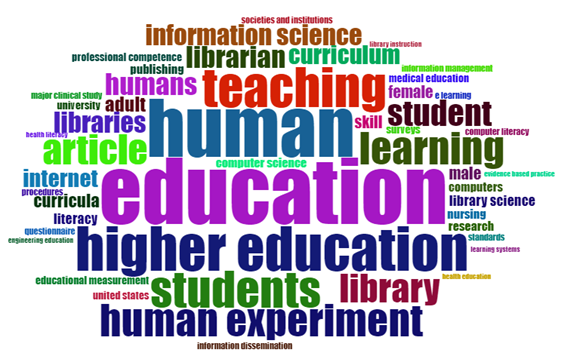
\includegraphics[width=0.6\textwidth]{fig5.png}
 \caption{Palabras clave más frecuentadas en la muestra de artículos.}
 \label{fig5}
 \source{Elaboración propia.}
\end{figure}

\section{Discusión}
La irrupción de la tecnología ha provocado que las formas de recabar información hayan sido modificadas en favor de  plataformas digitales como las redes sociales y las páginas webs \cite{alonsoelat2020}. %(ALONSO ET AL, 2020). 
Como consecuencia, fenómenos desinformativos como las \emph{fake news} se encargan de difundir mensajes confusos y manipulados de forma inmediata a toda una sociedad.

Ante esta situación que está generando desconcierto y preocupación en la sociedad, la pertinencia de la alfabetización informacional y la formación en competencias informacionales se ha presentado como uno de los desafíos educativos de los últimos años. Con esta antesala, el objetivo de este trabajo fue esclarecer cuál era el nivel de productividad acerca de alfabetización informacional en la etapa de Educación Superior en base a un diseño investigativo de carácter bibliométrico.

Con este propósito, los resultados hallados en el presente estudio, constataron la trascendencia de la línea de investigación en la actualidad, mostrando unos índices de productividad elevados, pese a la longevidad que presenta la línea de investigación desde su origen. Asimismo, los análisis de productividad en torno a institución y autores, permitió conocer la extensa variedad de autores procedentes de diferentes instituciones internacionales que se han dedicado a indagar sobre esta línea temática. Del mismo modo, los trabajos científicos que se encuentran en las principales revistas que publican sobre esta tópico poseen un gran índice de citación, y por ende, de impacto. Por lo tanto, se trata de una línea de investigación que suscita el interés de la comunidad científica y cuyos resultados son compartidos entre las diferentes plataformas divulgadoras. En este sentido, se establece una línea coincidente con lo expresado en estudios anteriores que evidencian estas palabras \cite{demeulemeesteretal2019, demeulemeester2018}. %(DE MEULEMEESTER ET AL, 2018; DE MEULEMEESTER, BUYSSE Y PELEMAN, 2018).

Por otro lado, el análisis de las principales temáticas proporcionó información valiosa acerca de la tipología de estudios que se abarca en torno a esta línea de investigación. Así, los resultados indicaron que predominan estudios de carácter evaluativo que se han encargado de analizar las percepciones y aptitudes informacionales en diferentes muestras de estudiantes. Se aboga por la necesidad de continuar en esta senda de investigación, pues resulta imprescindible seguir identificando los niveles de competencias informacionales existentes en los estudiantes para poder aplicar medidas resolutivas lo más pertinentes posibles. De esta manera, los trabajos acerca de la inclusión curricular de las competencias informacionales en los currículos educativos proporcionarán una enseñanza más contextualizada y funcional acorde a las necesidades presentes que demandan los estudiantes universitarios actuales \cite{ball2019, george2019}. %(BALL, 2019; GEORGE Y ROWLAND, 2019).  

En consiguiente, respecto a la evolución de la línea de investigación, el análisis cronológico reveló constructos que se encuentran muy relacionados con la alfabetización informacional, como fue el caso de la enseñanza online o Web 2.0. Se trata de descriptores muy relacionados y asociados a la alfabetización informacional, pues para poder desempeñar una navegación en la web responsable y adecuada, es fundamental poseer un nivel óptimo de conocimientos informacionales con respecto al mundo digital \cite{oecd2017}. %(OCDE, 2017).  
Finalmente, el análisis de palabras clave permitió corroborar aquella terminología más recurrente en la muestra de artículos y, de esta manera, corroborar la información otorgada en el análisis de temáticas. Los conceptos más frecuentados quedan vinculados al contexto educativo, lo cual radica la trascendencia de la formación en esta disciplina y la necesidad de continuar en su investigación e identificación de necesidades en este sentido.

\section{Conclusiones}
La actual sociedad del siglo XXI ha provocado que, en términos de información, vivamos en un periodo convulso, en el que las plataformas digitales publican cantidades exponenciales de noticias prácticamente al segundo. Esto provoca que la aparición de \emph{fake news} en la red sea un frecuente suceso, que, desafortunamente provoca un clima de confusión y crispación en la población.

En contraposición, y con la finalidad de confrontar este polémico fenómeno, la alfabetización informacional se presenta como una solución que se presenta como la principal panacea para combatir la desinformación existente en la red digital. A través de este trabajo se pretendió constituir un estado de la cuestión genérico acerca de los niveles de productividad existentes hasta el presente año en términos investigativos en las principales bases de datos científicas. Los resultados permitieron localizar los principales focos de productividad, así como las principales temáticas abordadas y características de los estudios.

Ante el abrumador volumen de nueva información científica, avances conceptuales y datos en el entorno, la bibliometría cobra utilidad al proporcionar un análisis estructurado a un gran conjunto de información, con la finalidad de inferir tendencias a lo largo del tiempo, temas investigadores, identifica cambios en los límites de las disciplinas, detectar a la mayoría de los académicos e instituciones de mayor índice prolífico y mostrar el estado general de la investigación existente en esta concreta temática \cite{aria2017}. %(ARIA, \& CUCCURULLO, 2017). 
Así, los resultados de este trabajo indicaron la todavía trascendencia y carácter emergente que aguarda a esta disciplina, común a diferentes disciplinas del conocimiento e instituciones de Educación Superior, así como la variedad existente de trabajos científicos vinculados a este tópico encontrado en los principales repositorios.

En referencia a las limitaciones del estudio, se encuentra la amplia muestra de trabajos escrutinados, que impidió poder establecer un análisis sistemático de ellos. Sin embargo, a partir de los métodos bibliométricos expuestos, se permitió establecer un estado general de la cuestión sobre la línea de investigación, que era el objetivo principal del trabajo. En cuanto a la prospectiva de trabajo, se aboga por la necesidad de continuar en el fomento en la formación en competencias informacionales, especialmente, desde la etapa de Educación Superior. Ante el vertiginoso y prolífico crecimiento de la información digital, resulta imprescindible que las próximas generaciones de profesionales estén dotados de aptitudes que le permitan convertirse en sujetos críticos a la hora de discernir fuentes de información y compartirla con el resto de la sociedad.

En conclusión, son múltiples los retos que afronta el sistema educativo ante los numerosos cambios experimentados a causa de la llegada de las tecnologías de la información y la comunicación. Ante esta situación, es fundamental que los futuros profesionales estén dotados de una formación de calidad, acorde a las necesidades que requiere la sociedad actual. Con esta finalidad, la Educación Superior debe emerger como aquella etapa educativa que ofrece recursos, estrategias y actitudes a los estudiantes de cara a afrontar los presentes y futuros desafíos sociales. Así, se promocionarán generaciones competentes y ambiciosas de cara a los múltiples desafíos futuros que depara a la sociedad.



%%%%%%%%%%%%%%%%%%%%%%%%%%%%%%%%%%%%%%%%%%%%%%%%%%%%%%%%%%%%%%%%%%%%%%%%%%%%%%%%%%%%%%%%%%%%%%%%%%%%%%%%%%%%%%%%%%%%%%%%%%%%%%%%%%%%%%%%%%%%%%%%%%%%%%%%%%%%%%%%%%%%%%%%%%%%%%%%%%%%%%%%%%%%%%%%%%%%%%%%%%%%%%%%%%%%%%%%%%%%%%%%%%%%%%%%%%%%%%%%%%%%%%%%%%%%%%%%%%%%%%%%%%%%%%%%%%%%%%%%%%%%%%%%%%%%%%%%%%%%%%%%%%%%%%%%%%%%%%%%%%%%%%%%%%%%%%%%%%%%%%



\printbibliography\label{sec-bib}
% if the text is not in Portuguese, it might be necessary to use the code below instead to print the correct ABNT abbreviations [s.n.], [s.l.] 
%\begin{portuguese}
%\printbibliography[title={Bibliography}]
%\end{portuguese}

\end{document}
